
\begin{figure}[t]
    \centering
    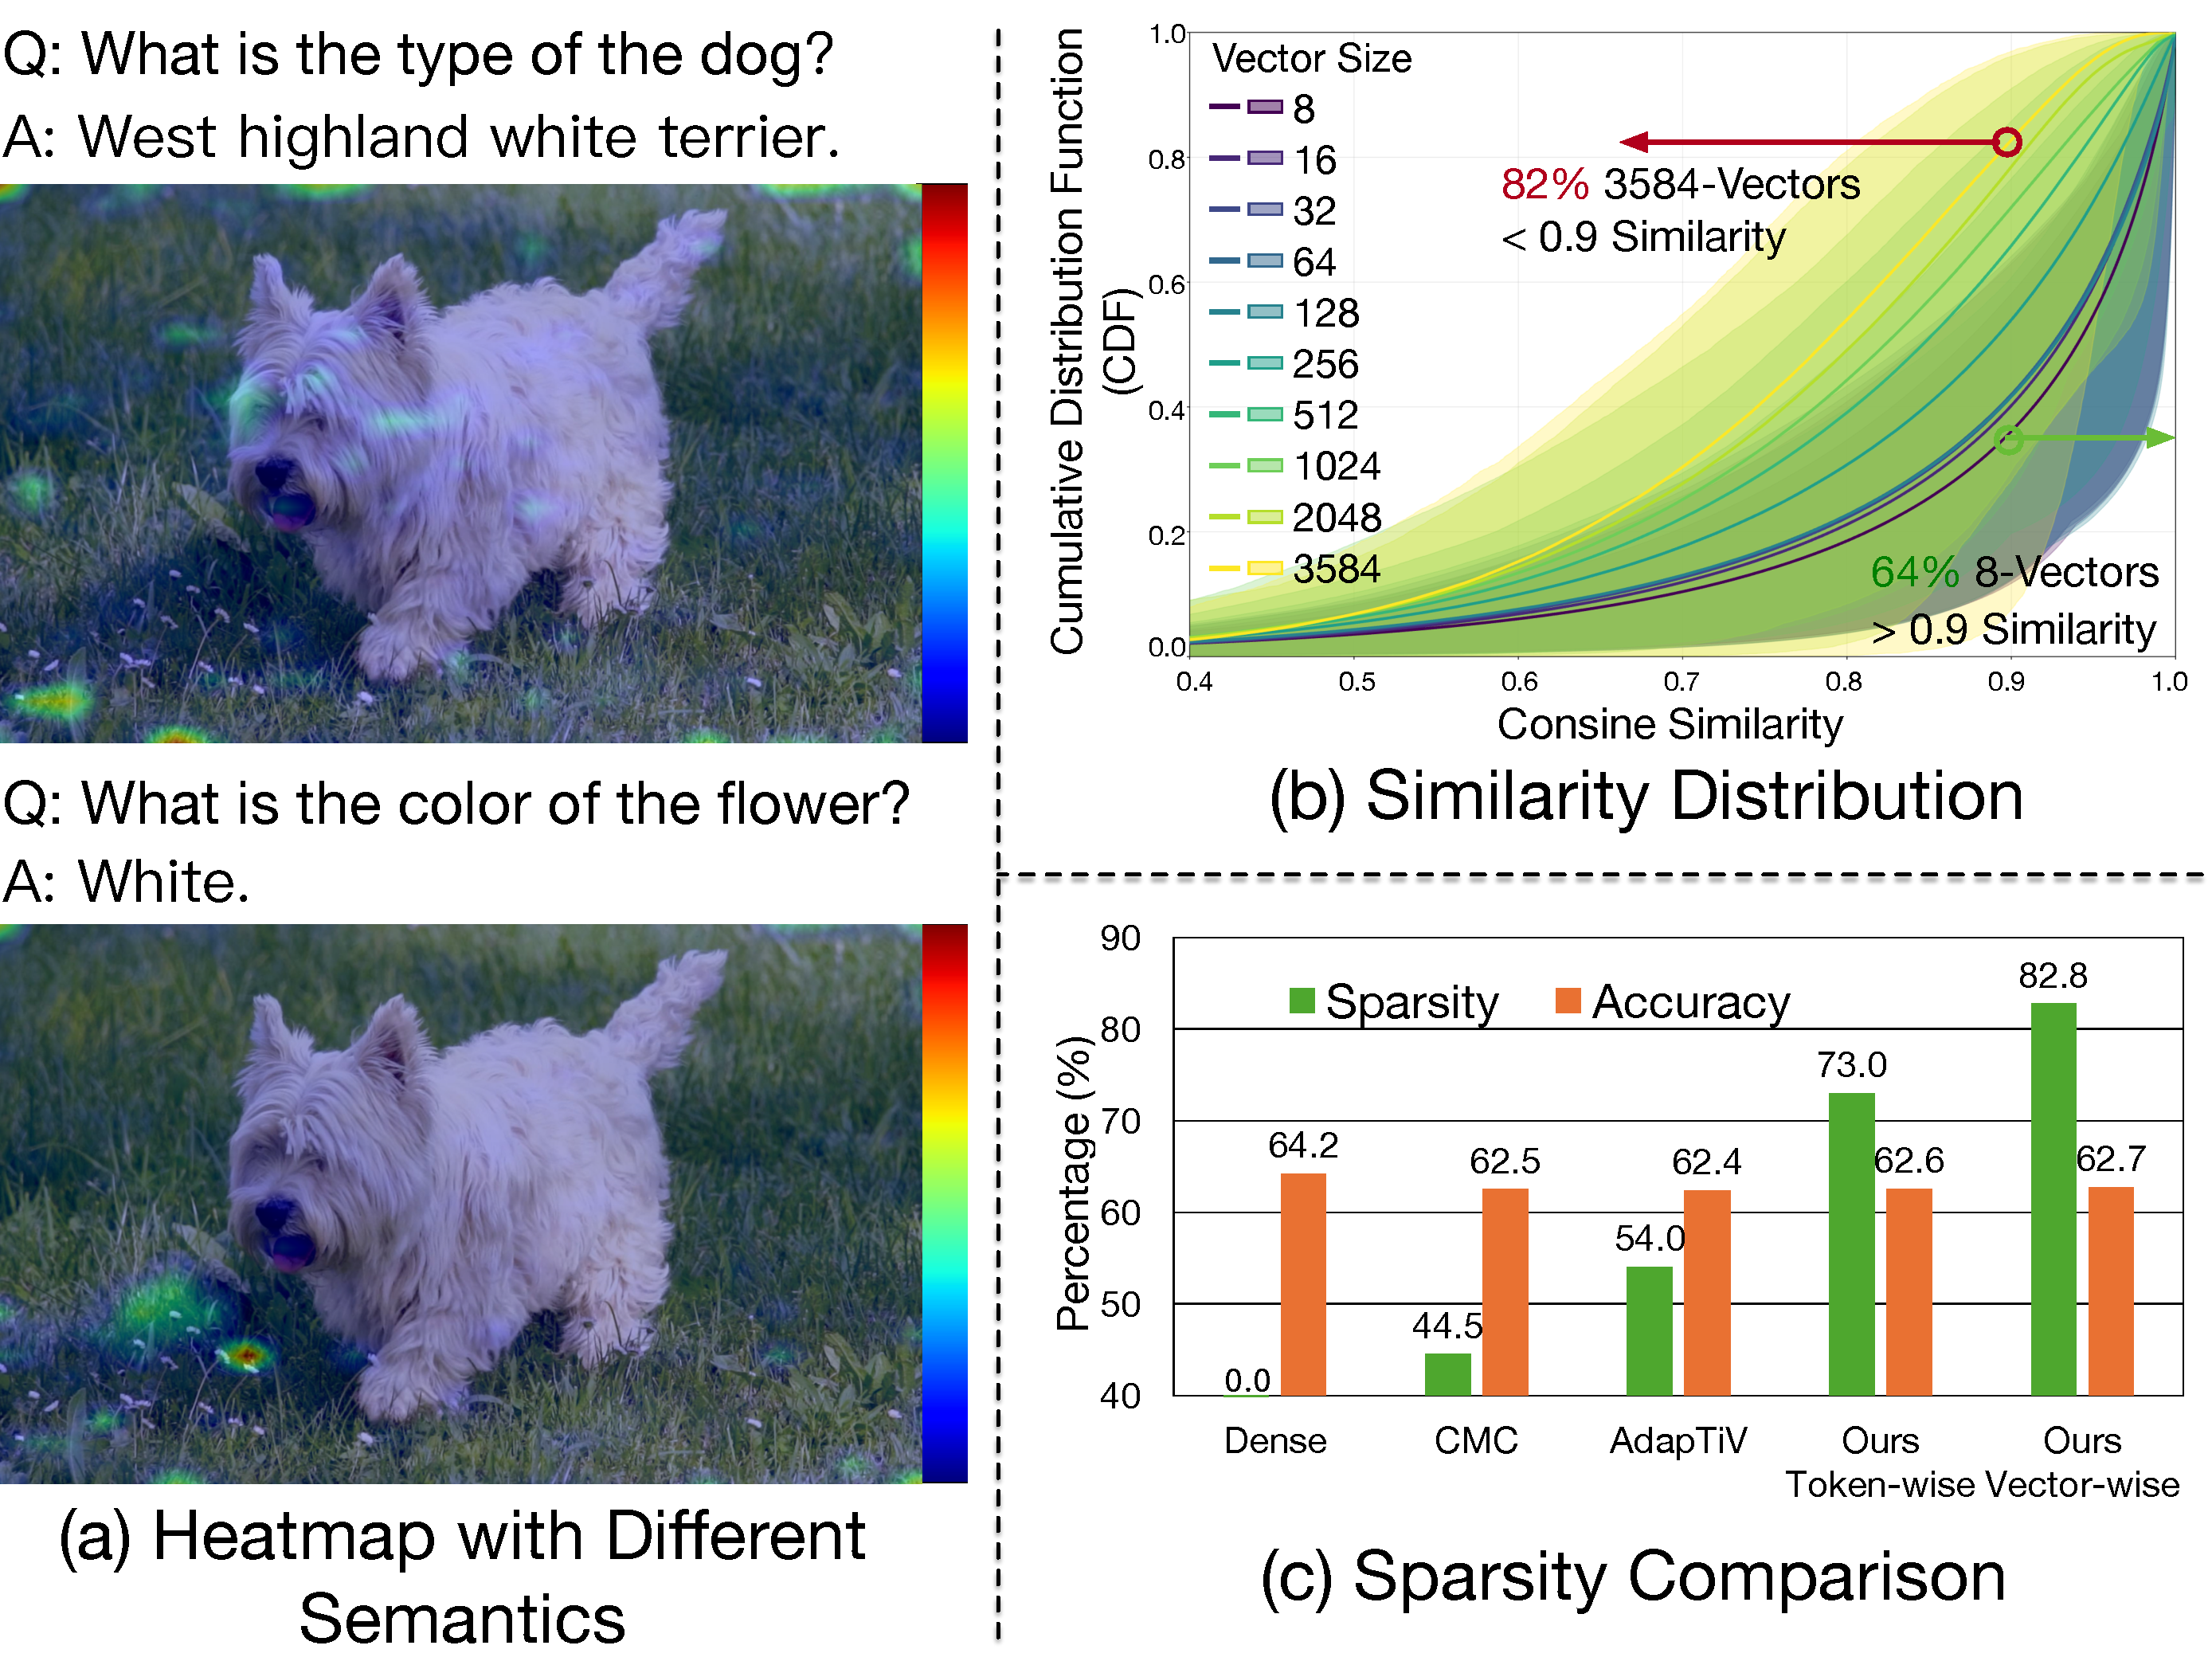
\includegraphics[width=1\linewidth]{figure/motivation1.pdf}
    % \vspace{-4mm}
    \caption{Motivation for multilevel concentration. 
    {(a) Prompt-aware attention heatmaps.} 
    {(b) Cosine similarity CDFs.} 
    (c) Sparsity Comparison.}
    \label{fig:motivation1}
    % \vspace{-5mm}
\end{figure}


\section{Motivation}
This section presents our motivation from both algorithmic and architectural perspectives across three levels:

(1) \textit{Token (semantic) level} prunes irrelevant tokens based on language context through semantic concentration;

(2) \textit{Block level (similarity scope)}  detects local spatiotemporal redundancy within adjacent regions using block-wise comparison;

(3) \textit{Vector level (similarity granularity)} captures fine-grained sub-token redundancy via vector-wise similarity.

\subsection{Algorithm: Multilevel Concentration}
\label{subsec:motivation_algo}
\textbf{Semantic Attention Shifts with the Prompt.}
In Vision-Language Models (VLMs), token importance is inherently tied to the input prompt. 
Prior pruning methods often rely on static heuristics such as saliency or token magnitude, which fail to capture prompt-specific semantic intent.

To illustrate this, we extract cross-modal attention maps {averaged from all layers} of the Llava-Onevision-7B~\cite{li2024llava} model under two different prompts, as shown in \Fig{fig:motivation1}(a). 
When asked \textit{``What is the type of the dog?''}, attention concentrates on the dog; when asked \textit{``What is the color of the flower?''}, attention shifts to the lower-left corner where the flowers reside. 
These examples highlight that semantically relevant tokens vary greatly with the question, and static importance metrics are inadequate.

Our semantic concentration module leverages cross-modal attention to prune uninformative tokens early, improving efficiency without degrading accuracy.

\textbf{Fine-grained Granularity Enhances Redundancy Detection.}  
Global token-level matching is often too coarse to capture redundancy arising from motion, deformation, or soft spatial shifts. 
As illustrated in \Fig{fig:intro}(c), a token in one frame may partially overlap with several neighboring tokens in the next frame, rendering single-token matching ineffective.

To better capture such partial alignments, we divide token embeddings into {vectors} and perform similarity comparisons at the vector level.
We extract {all layers' input} from Llava-OneVision~\cite{li2024llava} model with the MLVU~\cite{zhou2025mlvu} dataset.
{\Fig{fig:motivation1}(b) shows the average cosine similarity distribution across all layers, along with the variation range among layers. On average, over 64\% of 8-dimensional vectors exceed a cosine similarity threshold of 0.9, compared to only 18\% for 3584-dimensional vectors, indicating that finer granularity reveals substantially more redundancy.}
This enables higher sparsity without degrading accuracy.  
As shown in \Fig{fig:motivation1}(c), our vector-level method achieves 82.8\% sparsity on Llava-Video~\cite{zhang2024video} with the VideoMME~\cite{fu2025video} dataset, outperforming both CMC and AdapTiV, and exceeding our token-wise variant by 9.8\%. 
This translates to a 1.6$\times$ reduction in computation, while slightly improving accuracy.


Block- and vector-level strategies are complementary: block granularity defines \textit{where} comparisons are applied (e.g., within spatiotemporal windows), while vector granularity determines \textit{how fine} those comparisons are conducted.  
Together, they yield structured sparsity that aligns naturally with GEMM tiling, enabling efficient and accurate compression in hardware.




\begin{figure}[t]
    \centering
    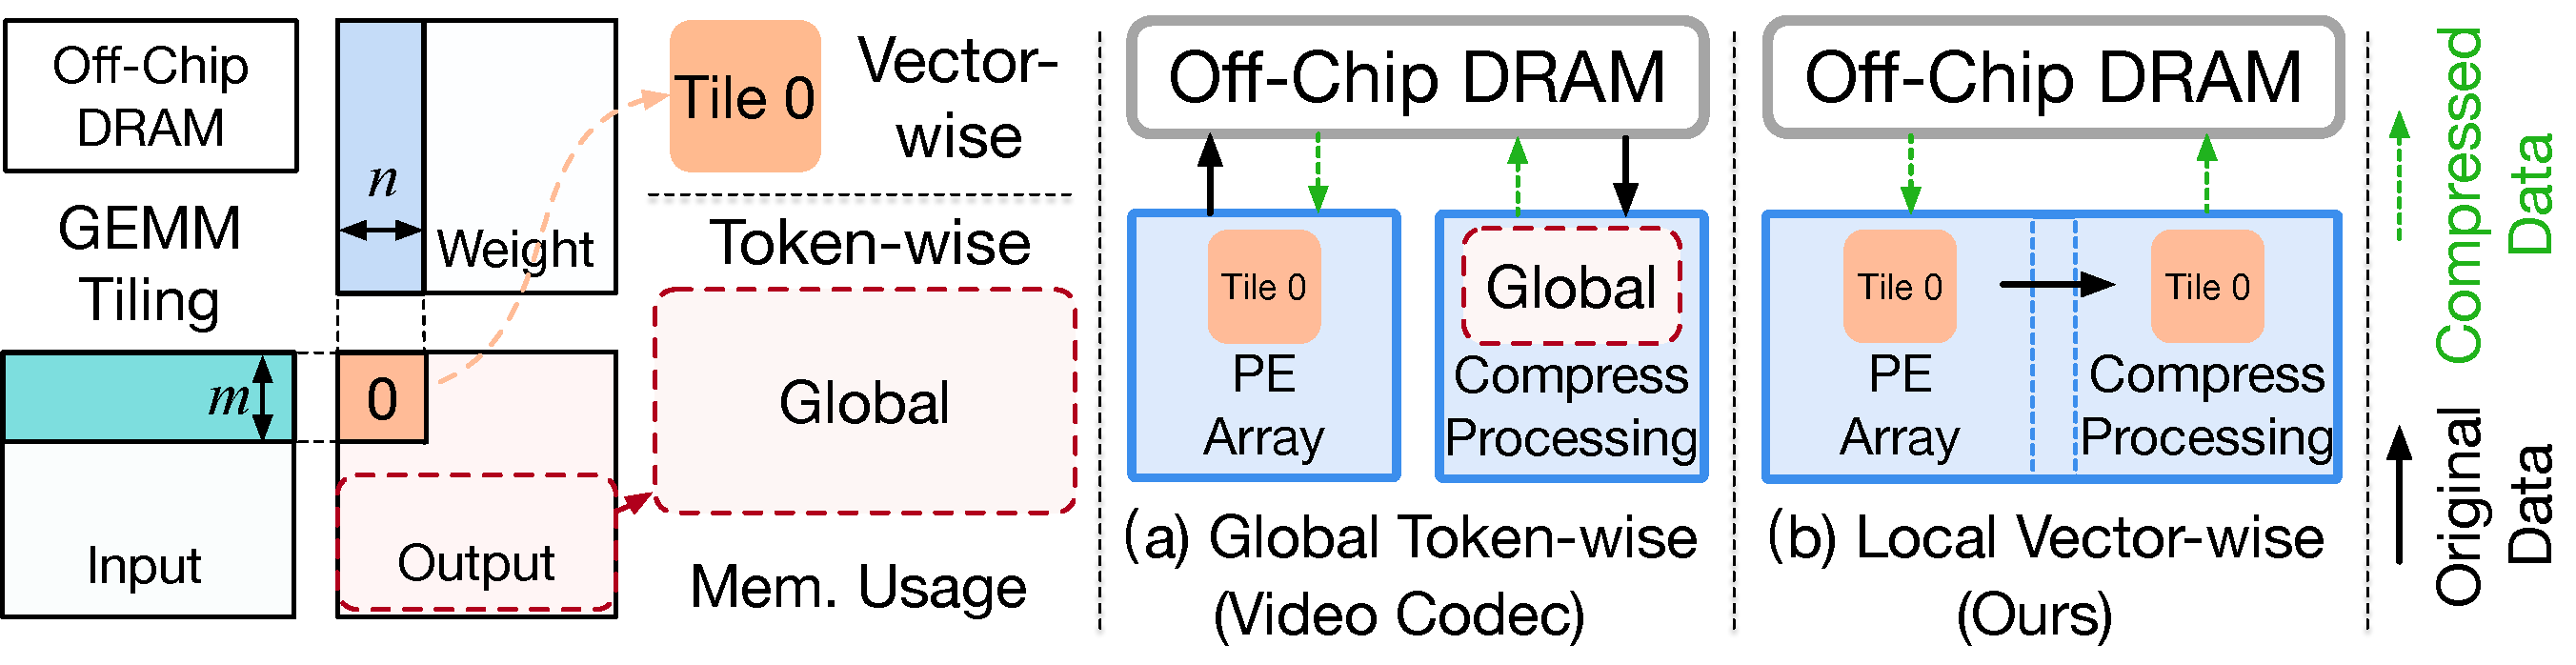
\includegraphics[width=1\linewidth]{figure/motivation2.pdf}
    % \vspace{-4mm}
    \caption{
    (a) Global token-wise methods (e.g., CMC) perform compression off-chip after writing all token outputs to DRAM. 
    (b) \proj{} compresses locally and on-chip at the vector level, immediately after each tile is produced. 
    }
    \label{fig:motivation2}
    % \vspace{-5mm}
\end{figure}


\subsection{Architecture: Hardware-Oriented Design}
While many efforts aim to improve VLM efficiency~\cite{bolya2023token,fu2024framefusion,liu2025nvila}, most focus on algorithmic techniques while overlooking hardware constraints.  
In high-throughput systems, algorithm and architecture must be co-designed, otherwise, even efficient algorithms can suffer from memory bottlenecks or poor data locality.  
As shown in \Fig{fig:motivation2}, our design bridges this gap through a \textbf{vector-wise compression strategy} that improves both accuracy and system efficiency.

\textbf{Limitations of Global Token-Wise Methods.}  
Prior designs like CMC~\cite{song2024cmc} adopt global, token-wise compression by offloading redundancy removal to a codec unit after writing full token outputs to DRAM~(\Fig{fig:motivation2}a).  
This incurs high bandwidth usage and sacrifices data locality.  
AdapTiV~\cite{yoo2024adaptiv} integrates token merging into hardware, but still relies on coarse token-pair operations and must transfer uncompressed tokens before processing.
{If prior designs were required to perform compression before writing back to DRAM, they would need an additional large buffer; for example, CMC uses up to 1.4MB.}
Token-wise methods also require full-token readiness before redundancy detection, limiting streaming.

Moreover, these approaches overlook sub-token redundancy and operate at the full GEMM level, which misaligns with the execution model of systolic arrays that process small, regular GEMM tiles.
Their global execution prevents fine-grained scheduling and increases memory pressure.  
As shown in \Sec{sec:mem_access}, CMC achieves 46\% sparsity but still incurs 79\% of dense DRAM traffic, whereas \proj{} reaches 81\% sparsity with only 21\% of the bandwidth, highlighting the advantage of hardware-aligned, vector-level concentration.


\textbf{GEMM-Tile Friendly Compression.}  
\proj{} performs compression entirely within each GEMM tile, aligning with the compute flow of systolic arrays.  
As shown in \Fig{fig:motivation2}(b), vector-level similarity is computed immediately after generating each $m \times n$ tile, using on-chip logic with no off-chip access.
This tile-local design preserves output regularity, introduces structured sparsity, and minimizes control and data movement overhead, making it naturally hardware-efficient.

We further adopt a block-wise scheduling strategy using sliding windows.  
Each block is processed in-stream, enabling local reuse and eliminating the need for global buffering.  
Our conflict-free memory layout (\Sec{subsec:layout}) supports parallel compression units without access contention, allowing \proj{} to scale with tile throughput at negligible latency.

In summary, \proj{} demonstrates effective {hardware-algorithm} co-optimization. 
Our vector-wise design improves redundancy detection and model fidelity, while streaming and tile-local execution ensure high hardware efficiency. 
This tightly integrated architecture makes \proj{} scalable, practical, and deployable for real-world VLM applications.
